\chapter{Implementación computacional de las bases discretas de Legendre}
\label{Implementación computacional de las bases discretas de Legendre en Python}

Haciendo uso de
la fórmula establecida en el teorema
\ref{teo: expresión analítica de BON de Legendre}
y las simetrías exploradas en el capítulo
\ref{section: sobre simetrias en las entradas de los poliomios discretos de Legendre}, definiremos un
algoritmo en el que
implementamos computacionalmente
las bases de Legendre discretas. Para probarlo, lo escribiremos
en Python. 
El input y output del algoritmo deseado son como siguen:


\begin{itemize}
\item \textbf{Input}: la dimensión requerida $n \geq 2$, variable
de tipo \code{int}. 
\item \textbf{Output}: lista con $n$ entradas,
siendo la $k-$ésima entrada (con $0 \leq k \leq n-1$)
una lista que contiene las $n$ entradas del
vector $\cali{L}^{n,k}$.
\end{itemize}

\begin{figure}[H]
	\sidecaption{
	Se ilustran el input y el output
		esperados del algoritmo para $n=5$. En el programa
		que escribimos más abajo
		no se pidió redondeo a cuatro decimales.
	\label{fig: input y output deseados}
	}
	\centering
	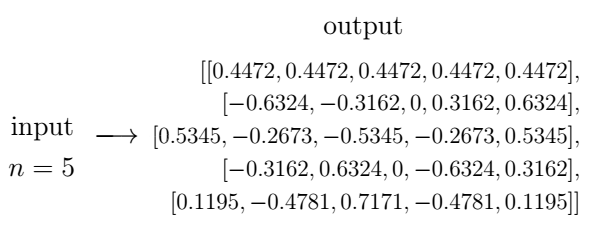
\includegraphics[scale=0.7]{7En_1} 
\end{figure}	

Sean $n \in \IN$, $0 \leq k \leq n-1$.
Veamos cómo usar lo que sabemos para calcular eficientemente
al vector $\cali{L}^{n,k}$ o, equivalentemente, para calcular
cada una de sus $n$ entradas, que son los números reales
$\cali{L}^{n,k}_{m}$, con $0 \leq m \leq n-1$.

Conviene reescribir la expresión
\eqref{eq0: 6En} resaltando con colores el papel que juegan
la dimensión $n$, el grado $k$ y la posición $m$ en la fórmula
para $\cali{L}^{n,k}_{m}$:

\begin{equation}
\label{eq1: 6En}
\cali{L}^{
{\color{ameMorado}{n}},{\color{ameAzul}{k}}}_{\color{ameDorado}{m}}= 
(-1)^{{\color{ameAzul}{k}}} 
\sqrt{\frac{(2
{\color{ameAzul}{k}}+1)(
{\color{ameMorado}{n}}-1)^{(
{\color{ameAzul}{k}})}}{(
{\color{ameMorado}{n}}+
{\color{ameAzul}{k}})^{(
{\color{ameAzul}{k}}+1)}}}
\suma{j=0}{
{\color{ameAzul}{k}}}{(-1)^{j}\binom{
{\color{ameAzul}{k}}}{j}\binom{
{\color{ameAzul}{k}}+j}{j}
\frac{{\color{ameDorado}{m}}^{(j)}}{(
{\color{ameMorado}{n}}-1)^{(j)}}}.
\end{equation}

Recuerde el concepto de fading factorial
definido en \ref{def: fading factorial}.
Observe ahora que, en la expresión \eqref{eq1: 6En},
aparecen cuatro fading factorials;
\begin{itemize}
\item $(n-1)^{(k)}$, que nunca es cero, pues $n-1 \geq k$
siempre ocurre,
\item $(n+k)^{(k+1)}$, que nunca es cero, pues $n+k \geq k+1$
siempre ocurre,
\item $(n-1)^{(j)}$ que, por ocurrir $j \leq k \leq n-1$, 
nunca es cero, y
\item $m^{(j)}$, que no es cero si y sólo si $j \leq m$;
\end{itemize}
según este último punto, algunos de los sumandos
considerados en la sumatoria 
en \eqref{eq1: 6En} pueden ser cero; podemos
ajustar el limite superior de la sumatoria y llegar así a que
\begin{equation}
\label{eq2: 6En}
\cali{L}^{
{\color{ameMorado}{n}},{\color{ameAzul}{k}}}_{\color{ameDorado}{m}}= 
(-1)^{{\color{ameMorado}{k}}} 
\sqrt{\frac{(2
{\color{ameAzul}{k}}+1)(
{\color{ameMorado}{n}}-1)^{(
{\color{ameAzul}{k}})}}{(
{\color{ameMorado}{n}}+
{\color{ameAzul}{k}})^{(
{\color{ameAzul}{k}}+1)}}}
\suma{j=0}{
min(
{\color{ameAzul}{k}},
{\color{ameDorado}{m}})
}{
{(-1)^{j}\binom{
{\color{ameAzul}{k}}}{j}\binom{
{\color{ameAzul}{k}}+j}{j}
\frac{{\color{ameDorado}{m}}^{(j)}}{(
{\color{ameMorado}{n}}-1)^{(j)}}}.
},
\end{equation}

Podemos también usar la definición de fading factorial
para reescribir \eqref{eq2: 6En}
en términos de factoriales
como sigue:


\begin{equation}
\label{eq5: 6En}
\cali{L}^{
{\color{ameMorado}{n}},{\color{ameAzul}{k}}}_{\color{ameDorado}{m}}= 
A_{
{\color{ameMorado}{n}},
{\color{ameAzul}{k}}
}
\suma{j=0}{
min(
{\color{ameAzul}{k}},
{\color{ameDorado}{m}})}
{B_{
{\color{ameMorado}{n}},
{\color{ameAzul}{k}},
{\color{ameDorado}{m}},j
}
},
\end{equation}
donde

\begin{equation}
\label{eq3: 6En}
A_{
{\color{ameMorado}{n}},
{\color{ameAzul}{k}}
}:=
(-1)^{{\color{ameAzul}{k}}} 
({\color{ameMorado}{n}}-1)!
\sqrt{\frac{(2
{\color{ameAzul}{k}}+1)}
{(
{\color{ameMorado}{n}}-
({\color{ameAzul}{k}}+1))!
(
{\color{ameMorado}{n}} + {\color{ameAzul}{k}}
)!
}},
\end{equation}
y

\begin{equation}
\label{eq4: 6En}
B_{
{\color{ameMorado}{n}},
{\color{ameAzul}{k}},
{\color{ameDorado}{m}},j
}:=
(-1)^{j}
\frac{
{\color{ameDorado}{m}}!
}{
({\color{ameMorado}{n}}-1)!
}
\frac{
({\color{ameAzul}{k}} + j) !
({\color{ameMorado}{n}}-(j+1))!
}{
(j!)^{2}
({\color{ameAzul}{k}}-j)!
({\color{ameDorado}{m}}-j)!
}.
\end{equation}



Usando las fórmulas \eqref{eq5: 6En}, 
\eqref{eq3: 6En} y \eqref{eq4: 6En} junto con las
simetrías estudiadas en la sección 
\ref{section: sobre simetrias en las entradas de los poliomios discretos de Legendre}, podemos escribir con facilidad el algoritmo deseado.

\subsection{Pseudocódigo de un algoritmo que calcula bases de Legendre discretas}
A continuación mostramos los pseudocódigos para calcular 
los polinomios discretos de Legendre.

\begin{itemize}
\item Damos dos algoritmos (\TODO{citas}) para calcular el número
\begin{equation}
\label{eq0: 1Abril}
B_{n, k, m, j};
\end{equation}
el primero usa directamente la fórmula \eqref{eq4: 6En},
mientras que en el segundo 
simplificamos los factoriales que
aparecen en la definición \eqref{eq4: 6En}
de $B_{n,k,m,j}$
para llegar a la expresión
\[
(-1)^{j}
\frac{m!}{(n-1)!}
 \frac{(k+j)!(n-j-1)!}{(j!)^{2}(k-j)!(m-j)!}
= (-1)^{j}
\frac{\left( \producto{\mu=m-j+1}{m}{\mu} \right)
\left( \producto{\mu=k-j+1}{k+1}{\mu} \right)
}{
\left( \producto{\mu=n-j}{n-1}{\mu} \right)
\left( \producto{\mu=n-j}{n-1}{\mu} \right)^{2}
}
\]
y, para simplificar aún más los cálculos, el algoritmo
busca qué factores se repiten en el numerador y en el denominador,
para así eliminarlos y sólo calcular el producto de los 
números restantes.
\item Damos dos algoritmos (\TODO{ref}) para calcular a la suma
\begin{equation}
\label{eq1: 1Abril}
\suma{j=0}{min(k,m)}{B_{n, k, m, j}};
\end{equation}
\TODO{di cuál se corresponde con cuál.}
\item Los algoritmos \TODO{ref} para calcular, usando alguna
de las dos versiones de ``sumatoria'', la base de Legendre discreta
de dimensión $n$.
\end{itemize}

Observe cómo
en los algoritmos \ref{alg: legendre Impar} y \ref{alg: legendre Par}
primero iteramos sobre $k$, la variable de grado, y
luego sobre $m$, la variable de posición. \TODO{No me gusta usar
$\leftarrow$ para cambiar los números almacenados en vector legendre.}.
Las lineas 10 de estos 
algoritmos 
se justifican,
respectivamente, con los teoremas \ref{prop: simetrias en dimensiones impares}
y \ref{prop: simetrias en dimensiones pares}.


\begin{algorithm}
\caption{$sumandoV1$}
\begin{algorithmic} [1]
\REQUIRE $n$, $k$, $m$, $j$, todas de tipo int, con $n \geq 2$, 
$0 \leq k, m \leq n-1$, $0 \leq j \leq min(k,m)$
\ENSURE El número \eqref{eq0: 1Abril}
\RETURN $\frac{(k+j)! * (n-j-1)! }{(j!)^{2}* (k-j)! * (m-j)!}$
\end{algorithmic}
\end{algorithm}


\begin{algorithm}
\caption{$sumatoriaV1$}
\begin{algorithmic} [1]
\REQUIRE $n$, $k$, $m$, $j$, todas de tipo int, con $n \geq 2$, 
$0 \leq k, m \leq n-1$, $0 \leq j \leq min(k,m)$
\ENSURE El número \eqref{eq0: 1Abril}

\STATE $limite \leftarrow minimo(m,k)$
\STATE $factor \leftarrow \frac{m!}{(n-1)!}$
\STATE $sumandos_pares \leftarrow []$
\STATE $sumandos_impares \leftarrow []$
\FOR {$j=0$ a $j=limite$ y $j$ par} 
\STATE $APPEND$($sumandos\_pares$, $sumandoV1(n,k,m,j)$)
\ENDFOR
\FOR {$j=0$ a $j=limite$ y $j$ impar} 
\STATE $APPEND$($sumandos\_impares$, $sumandoV1(n,k,m,j)$)
\ENDFOR
\STATE $suma\_pares \leftarrow SUM(sumandos\_pares)$
\STATE $suma\_impares \leftarrow SUM(sumandos\_impares)$
\RETURN $factor * (suma\_pares - suma\_impares)$
\end{algorithmic}
\end{algorithm}


\begin{algorithm}
\caption{AAA}
\begin{algorithmic}[1] 
\REQUIRE $n$, $k$, $m$ todas de tipo int, con $n \geq 2$, 
$0 \leq k, m \leq n-1$.
\ENSURE la sumatoria que aparece en el lado derecho de la
ecuación \eqref{eq5: 6En}
para los correspondientes valores de $n$, $k$ y $m$.

\STATE $limite \leftarrow minimo(m,k)$
\STATE $factor \leftarrow \frac{m!}{(n-1)!}$
\STATE $suma \leftarrow 0$
\FOR {$j=0$ a $j=limite$} 
\STATE $suma \leftarrow suma + 
(-1)^{j} \frac{(k+j)!(n-j-1)!}{(j!)^{2}(k-j)!(m-j)!}$
\ENDFOR
\STATE $resultado \leftarrow factor*suma$
\RETURN $resultado$
\end{algorithmic}
\end{algorithm}

%-----------------------------------------------------------------

\begin{algorithm}
\caption{base$\_$legendre$\_$dimImpar}\label{alg: legendre Impar}
\begin{algorithmic}[1] 
\REQUIRE $n$, variable de tipo int, $n \geq 2, \hspace{0.1cm} n \equiv 1 \hspace{0.1cm} (mod \hspace{0.1cm} 2)$
\ENSURE lista cuyos elementos son $n$ listas, conteniendo
la $k-$ésima lista las $n$ entradas del polinomio discreto de Legendre de
grado $k$ y dimensión $n$.
%\ENSURE $y = x^n$
\STATE $N \leftarrow n//2$
\STATE $base\_legendre=[ \hspace{0.2cm} ]$ 

\FOR {$k=0$ a $k=n-1$} 
\STATE $A\_nk \leftarrow (-1)^{k}*(n-1)!*
\sqrt{\frac{
2k+1
}{
(n-k-1)!*(n+k)!
}}$

\STATE $vector\_legendre \leftarrow [ 0, \ldots , 0]$ \COMMENT{Lista con $n$ ceros} 
\FOR {$m=0$ a $m=N-1$} 
\STATE $suma \leftarrow sumatoria(n,k,m)$
\STATE $entrada\_legendre=A\_nk * suma$
\STATE $vector\_legendre[m] \leftarrow entrada\_legendre$ 
\STATE $vector\_legendre[2N-m] \leftarrow (-1)^{k}*entrada\_legendre$ 
\ENDFOR

\IF{$k \equiv 1 \hspace{0.1cm} (mod \hspace{0.1cm} 2)$}
\STATE $vector\_legendre[N] \leftarrow 0$
\ELSE
\STATE $suma \leftarrow sumatoria(n,k,N)$
\STATE $vector\_legendre[N] \leftarrow (-1)^{k}*A\_nk * suma$
\ENDIF
\STATE Agregar $vector\_legendre$ a la lista $base\_legendre$
\ENDFOR
\RETURN $base\_legendre$
\end{algorithmic}
\end{algorithm}



\begin{algorithm}
\caption{base$\_$legendre$\_$dimPar}\label{alg: legendre Par}
\begin{algorithmic} [1]
\REQUIRE $n$, variable de tipo int, $n \geq 2, \hspace{0.1cm} n \equiv 0 \hspace{0.1cm} (mod \hspace{0.1cm} 2)$
\ENSURE lista cuyos elementos son $n$ listas, conteniendo
la $k-$ésima lista las $n$ entradas del polinomio discreto de Legendre de
grado $k$ y dimensión $n$.


\STATE $N \leftarrow n//2$
\STATE $base\_legendre=[ \hspace{0.2cm} ]$

\FOR {$k=0$ a $k=n-1$} 
\STATE $A\_nk \leftarrow (-1)^{k}*(n-1)!*
\sqrt{\frac{
2k+1
}{
(n-k-1)!*(n+k)!
}}$

\STATE $vector\_legendre \leftarrow [ 0, \ldots , 0]$ \COMMENT{Lista con $n$ ceros} 
\FOR {$m=0$ a $m=N-1$} 
\STATE $suma \leftarrow sumatoria(n,k,m)$
\STATE $entrada\_legendre=A\_nk * suma$
\STATE $vector\_legendre[m] \leftarrow entrada\_legendre$ \COMMENT{Agregamos en la $m-$ésima posición}
\STATE $vector\_legendre[2N-m-1] \leftarrow (-1)^{k}*entrada\_legendre$
\ENDFOR


\STATE Agregar $vector\_legendre$ a la lista $base\_legendre$
\ENDFOR
\RETURN $base\_legendre$
\end{algorithmic}
\end{algorithm}



\begin{algorithm}
\caption{Calcular la base de Legendre de dimensión $n$}
\begin{algorithmic} [1]
\REQUIRE $n$, variable de tipo int, $n \geq 2$.
\ENSURE lista cuyos elementos son $n$ listas, conteniendo
la $k-$ésima lista las $n$ entradas del polinomio discreto de Legendre de
grado $k$ y dimensión $n$.

\IF{$n \equiv 0 \hspace{0.1cm} (mod \hspace{0.1cm} 2)$}
\STATE $base\_legendre\_dimPar(n)$
\ELSE
\STATE $base\_legendre\_dimImpar(n)$
\ENDIF
\end{algorithmic}
\end{algorithm}

\subsection{Código en Python}
\TODO{Recuerda cambiar el código para usar np.arrays.
Vectorizar datos?}



Para empezar, damos dos algoritmos que pueden
usarse para calcular la sumatoria 
\[
\suma{j=0}{min(k,m)}{B_{n,k,m,j}}.
\] 
Uno de ellos usa
directamente la expresión \eqref{eq4: 6En}, mientras
que en el otro se simplifican los factoriales que
aparecen en la definición \eqref{eq4: 6En}
de $B_{n,k,m,j}$
para llegar a la expresión
\[
(-1)^{j}
\frac{m!}{(n-1)!}
 \frac{(k+j)!(n-j-1)!}{(j!)^{2}(k-j)!(m-j)!}
= (-1)^{j}
\frac{\left( \producto{\mu=m-j+1}{m}{\mu} \right)
\left( \producto{\mu=k-j+1}{k+1}{\mu} \right)
}{
\left( \producto{\mu=n-j}{n-1}{\mu} \right)
\left( \producto{\mu=n-j}{n-1}{\mu} \right)^{2}
}
\]
y, para simplificar aún más los cálculos, el algoritmo
busca qué factores se repiten en el numerador y en el denominador,
para así eliminarlos y sólo calcular el producto de los 
números restantes. Observe que en ambos algoritmos, antes
de realizar la suma se calculan y guardan todos los sumandos
en una lista, pues queremos antes ordenarlos de menor a mayor.
\TODO{explica por qué.}
\TODO{termina de escribir los pseudocódigos.}

\TODO{Recuerda que debes explicar que ordenas
de menor a mayor para evitar lo más que se pueda errores
de redondeo. Puedes citar el artículo de la Recherche.}

